\documentclass[notes=show, 10pt, xcolor=table]{beamer}
\usepackage[utf8]{inputenc}
\usepackage{xeCJK}
\usepackage{graphicx}
\usepackage {mathtools}
\usepackage{multicol}
\usepackage{utopia} %font utopia imported
\usetheme{CambridgeUS}

\usepackage{booktabs}
\usepackage{multirow}
%\usepackage[table,xcdraw]{xcolor}

\usecolortheme{dolphin}

% set colors
\definecolor{myNewColorA}{RGB}{126,12,110}
\definecolor{myNewColorB}{RGB}{165,85,154}
\definecolor{myNewColorC}{RGB}{203,158,197}
\setbeamercolor*{palette primary}{bg=myNewColorC}
\setbeamercolor*{palette secondary}{bg=myNewColorB, fg = white}
\setbeamercolor*{palette tertiary}{bg=myNewColorA, fg = white}
\setbeamercolor*{titlelike}{fg=myNewColorA}
\setbeamercolor*{title}{bg=myNewColorA, fg = white}
\setbeamercolor*{item}{fg=myNewColorA}
\setbeamercolor*{caption name}{fg=myNewColorA}
\usefonttheme{professionalfonts}
\usepackage{natbib}
\usepackage{hyperref}
%------------------------------------------------------------
\titlegraphic{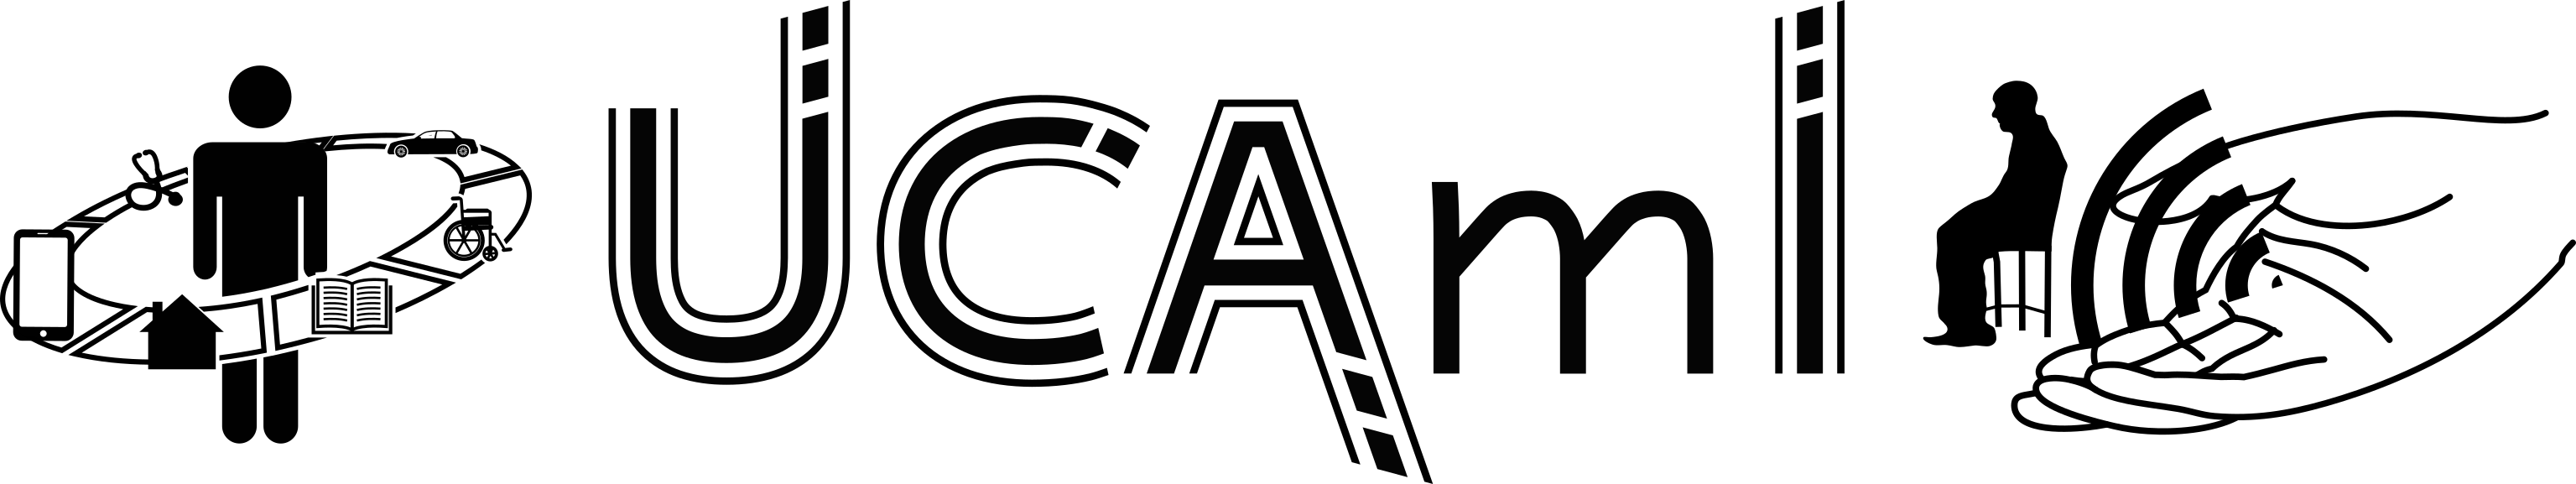
\includegraphics[height=1.5cm]{ucami2022.png}}

\setbeamerfont{title}{size=\large}
\setbeamerfont{subtitle}{size=\small}
\setbeamerfont{author}{size=\small}
\setbeamerfont{date}{size=\small}
\setbeamerfont{institute}{size=\small}

%\setbeameroption{show notes on second screen=right}

\title[UCAmI 2022]{Internet of Things (IoT)-Based System for Classroom Access Control and Resource Management}
\subtitle{(SISGERA)}
\author[Gleiston Guerrero-Ulloa]{Gleiston Guerrero-Ulloa \and Jonathan Villafuerte-Solorzano \and Michael Yánez  \and \\Miguel J. Hornos \and Carlos Rodriguez-Domínguez}

\institute[gguerrero@uteq.edu.ec]{Technical State University of Quevedo, and University of Granada}
\date[Córdoba, November 2022]{Córdoba, November 2022}

%------------------------------------------------------------
%This block of commands puts the table of contents at the 
%beginning of each section and highlights the current section:
%\AtBeginSection[]
%{
%  \begin{frame}
%    \frametitle{Contents}
%    \tableofcontents[currentsection]
%  \end{frame}
%}
\AtBeginSection[]{
  \begin{frame}
  \vfill
  \centering
  \begin{beamercolorbox}[sep=8pt,center,shadow=true,rounded=true]{title}
    \usebeamerfont{title}\insertsectionhead\par%
  \end{beamercolorbox}
  \vfill
  \end{frame}
}
%------------------------------------------------------------

\begin{document}

%The next statement creates the title page.
\frame{\titlepage}
\begin{frame}
\frametitle{Contents}
\tableofcontents
\end{frame}
%------------------------------------------------------------
\section{Introduction}
    \begin{frame}{Introduction}
        \begin{block}{What is SISGERA}
            SISGERA (from Spanish: SIStema de GEstión de Recursos de Aula) is a prototype of an IoT-based system that was developed as a possible and feasible solution to management of classroom resources, and as a consecuence reduce energy consumption.
        \end{block}
        In this work we aim to achieve three goals:
        \begin{block}{Aims}
            \begin{enumerate}
                \item With SISGERA, to improve management of classroom resources and
                \item Reducing electrical energy consumption, and
                \item Assessment the TDDM4IoTS (Test-Driven Development Methodology for IoT-based Systems) methodology
            \end{enumerate}
        \end{block}
    
        \begin{block}{Results}
            \begin{itemize}
                \item IoT Device
                \item Mobile application
                \item Methodology assessment
            \end{itemize}
        \end{block}
        \note{
            In this work we propose to SISGERA from Spanish: SIStema de GEstión de Recursos de Aula. SISGERA is a prototype of an IoT-based system that was developed following the Test-Driven Development Methodology for IoT-based Systems, as a possible and feasible solution to manage classroom resources and to control access to classrooms. Therefore, the present work has a three goals. The \textbf{first goal} Classroom resource management aims to ensure that classroom resources are switched on for the required time. And as a consequence, \textbf{the second goal} reduce energy consumption. And \textbf{last goal} evaluate the TDDM4IoTS.
            
            TDDM4IoTS is a methodology consisting of 11 phases, namely: Stage 1 Preliminary analysis, Stage 2 Technology layer design, Stage 3 Detailed requirement analysis, Stage 4 Model generation and adaptation, Stage 5 Test generation, Stage 6 Software generation, Stage 7 Model refinement, Stage 8 Software refinement, Stage 9 Hardware and software deployment, Stage 10 Deliverable assessment, and Stage 11 Maintenance. It addresses the development of both the software for IoT hardware configuration and the software for user interaction.
            }
    \end{frame}
\section{Goal (1): Improve management of classroom resources}
    \begin{frame}{Classroom resources}
        \begin{block}{Current challenges}
            \begin{itemize}
                \item The janitorial staff is in charge of opening the doors and turning on and off the appliances, and if it is the first hour, turning on the lights, and if it is the last hour, turning them off.
                \item Each janitorial staff member must control access to approximately 16 classrooms.
                \item On some days of the week, all classrooms start classes at the same time.
                \item The professor must record student attendance.
                \item The professor does not know all his students (at least for the first few class meetings).
            \end{itemize}
        \end{block}
        \begin{block}{Other challenges}
            \begin{itemize}
                \item The professor and students may leave the classroom at any time (e.g., when they need to move to practice labs).
                \item The professor does not have access to the remote controls of the devices.
            \end{itemize}
        \end{block}
        \note{
           The janitorial staff is in charge of opening the doors of each classroom at the beginning of the school shift in the morning and closing them at the end of the school shift in the afternoon. They to managing the door locks, they are in charge of the remote controls to manage classroom equipment such as projectors and air conditioners, so they turn these on at the beginning of the shift and expect to turn them off at the end of the shift. However, some professors turn them off at the end of their class session, leaving the next professor to contact staff to turn on or turn off the equipment they do not require.
           
           It is a rule that the classroom must be opened when the professor is ready to enter, which can be a delay or rush for the janitorial staff, as one day all classrooms will be required at the same time by the respective professors to start classes.
           
           When classes start, the professor must register the student's attendance, and from the very first classes, students may be evaluated on their performance, and the professor does not always identify each student, which may lead to some impersonation.
        }
    \end{frame}

\section{Goal (2): Reducing electrical energy consumption}
    \begin{frame}{Reducing electrical energy consumption}
        \begin{block}{{Careers offered by the Faculty of Engineering Sciences (FCI)}}
            \begin{itemize}
                \item Systems Engineering (currently, Software Engineering),
                \item Electrical Engineering,
                \item Mechanical Engineering, and
                \item Environmental Engineering
            \end{itemize}
        \end{block}
        
        \begin{block}{Types of teaching}
            \begin{itemize}
                \item Teorical
                \item Practical
            \end{itemize}
        \end{block}
        
        \begin{block}{Academic planning}
            At FCI of the UTEQ, classes are held in two shifts per day
            \begin{itemize}
                \item In the morning from 07:30 to 12:30
                \item In the afternoon from 12:30 to 17:30
            \end{itemize}
        \end{block}
        \note{
            The SISGERA prototype is implemented in a classroom at the Faculty of Engineering Sciences FCI. The FCI offers technical programs such as Electrical Engineering, Software Engineering, Mechanical Engineering and Environmental Engineering. Each course has only one professor in charge. Some courses of these programs have practical hours -laboratory or field- and theoretical hours, and the professor is in charge of planning when he/she will teach the theoretical classes and when the practical classes will take place.
            
            Every day there are two shifts of classes:
            \begin{itemize}
                \item in the morning from 07:30 to 12:30 and 
                \item from 12:30 to 17:30
            \end{itemize}
        }
    \end{frame}
    
    \begin{frame}{Reducing electrical energy consumption...}
        \begin{block}{Example classroom FCI-008 class schedule}
            \begin{table}[]
            	\begin{tabular}{@{}|l|l|l|l|l|l|@{}}
            		\toprule
            		\rowcolor[HTML]{303498} 
            		\multicolumn{1}{|c|}{\cellcolor[HTML]{303498}{\color[HTML]{FFFFFF} \textbf{\begin{tabular}[c]{@{}c@{}}Start time\\ to End time\end{tabular}}}} & {\color[HTML]{FFFFFF} \textbf{Monday}}                                & {\color[HTML]{FFFFFF} \textbf{Tuesday}}                               & {\color[HTML]{FFFFFF} \textbf{Wednesday}}        & {\color[HTML]{FFFFFF} \textbf{Thursday}}         & {\color[HTML]{FFFFFF} \textbf{Friday}}           \\ \midrule
            		\rowcolor[HTML]{9AFF99} 
            		07:30 – 0830                                                                                                                                   & \multicolumn{1}{c|}{\cellcolor[HTML]{9AFF99}}                         & \multicolumn{1}{c|}{\cellcolor[HTML]{9AFF99}}                         & \cellcolor[HTML]{FFFFFF}                         & \cellcolor[HTML]{9AFF99}                         & \cellcolor[HTML]{FFFFFF}                         \\ \cmidrule(r){1-1} \cmidrule(lr){4-4} \cmidrule(l){6-6} 
            		\rowcolor[HTML]{9AFF99} 
            		08:30 – 09:30                                                                                                                                  & \multicolumn{1}{c|}{\cellcolor[HTML]{9AFF99}}                         & \multicolumn{1}{c|}{\cellcolor[HTML]{9AFF99}}                         & \cellcolor[HTML]{FFFFFF}                         & \cellcolor[HTML]{9AFF99}                         & \cellcolor[HTML]{FFFFFF}                         \\ \cmidrule(r){1-1} \cmidrule(lr){4-4} \cmidrule(l){6-6} 
            		\rowcolor[HTML]{9AFF99} 
            		09:30 – 10:30                                                                                                                                  & \multicolumn{1}{c|}{\multirow{-3}{*}{\cellcolor[HTML]{9AFF99}ME9MC1}} & \multicolumn{1}{c|}{\multirow{-3}{*}{\cellcolor[HTML]{9AFF99}ME9MC3}} & \cellcolor[HTML]{9AFF99}                         & \multirow{-3}{*}{\cellcolor[HTML]{9AFF99}ME9MC6} & \cellcolor[HTML]{9AFF99}                         \\ \cmidrule(r){1-3} \cmidrule(lr){5-5}
            		\rowcolor[HTML]{9AFF99} 
            		10:30 – 11:30                                                                                                                                  & \cellcolor[HTML]{9AFF99}                                              & \cellcolor[HTML]{9AFF99}                                              & \cellcolor[HTML]{9AFF99}                         & \cellcolor[HTML]{9AFF99}                         & \multirow{-2}{*}{\cellcolor[HTML]{9AFF99}ME9MC4} \\ \cmidrule(r){1-1} \cmidrule(l){6-6} 
            		\rowcolor[HTML]{9AFF99} 
            		11:30 – 12:30                                                                                                                                  & \multirow{-2}{*}{\cellcolor[HTML]{9AFF99}ME9MC2}                      & \multirow{-2}{*}{\cellcolor[HTML]{9AFF99}ME9MC4}                      & \multirow{-3}{*}{\cellcolor[HTML]{9AFF99}ME9MC5} & \multirow{-2}{*}{\cellcolor[HTML]{9AFF99}ME9MC2} & \cellcolor[HTML]{FFFFFF}                         \\ \midrule
            		\rowcolor[HTML]{FFFC9E} 
            		12:30 – 13:30                                                                                                                                  & \cellcolor[HTML]{FFFFFF}                                              & \cellcolor[HTML]{FFFC9E}                                              & \cellcolor[HTML]{FFFC9E}                         & \cellcolor[HTML]{FFFFFF}                         & EE8MC5                                           \\ \cmidrule(r){1-2} \cmidrule(l){5-6} 
            		\rowcolor[HTML]{FFFC9E} 
            		13:30 – 14:30                                                                                                                                  & \cellcolor[HTML]{FFFC9E}                                              & \multirow{-2}{*}{\cellcolor[HTML]{FFFC9E}EE8MC3}                      & \multirow{-2}{*}{\cellcolor[HTML]{FFFC9E}EE8MC1} & \cellcolor[HTML]{FFFC9E}                         & EE8MC4                                           \\ \cmidrule(r){1-1} \cmidrule(lr){3-4} \cmidrule(l){6-6} 
            		\rowcolor[HTML]{FFFC9E} 
            		14:30 – 15:30                                                                                                                                  & \multirow{-2}{*}{\cellcolor[HTML]{FFFC9E}EE8MC1}                      & \cellcolor[HTML]{FFFC9E}                                              & \cellcolor[HTML]{FFFC9E}                         & \cellcolor[HTML]{FFFC9E}                         & \cellcolor[HTML]{FFFC9E}                         \\ \cmidrule(r){1-2}
            		\rowcolor[HTML]{FFFC9E} 
            		15:30 – 16:30                                                                                                                                  & \cellcolor[HTML]{FFFC9E}                                              & \cellcolor[HTML]{FFFC9E}                                              & \cellcolor[HTML]{FFFC9E}                         & \multirow{-3}{*}{\cellcolor[HTML]{FFFC9E}EE8MC3} & \cellcolor[HTML]{FFFC9E}                         \\ \cmidrule(r){1-1} \cmidrule(lr){5-5}
            		\rowcolor[HTML]{FFFC9E} 
            		16:30 – 17:30                                                                                                                                  & \multirow{-2}{*}{\cellcolor[HTML]{FFFC9E}EE8MC2}                      & \multirow{-3}{*}{\cellcolor[HTML]{FFFC9E}EE8MC4}                      & \multirow{-3}{*}{\cellcolor[HTML]{FFFC9E}EE8MC5} & EE8MC6                                           & \multirow{-3}{*}{\cellcolor[HTML]{FFFC9E}EE8MC6} \\ \bottomrule
            	\end{tabular}
            \end{table}
        \end{block}
        
        \note{
            As an example of a classroom use schedule, we provide below the morning shift schedule of the classroom, which is used to teach the ninth module of the Mechanical Engineering degree, is show in green.
            
            However, lessons are given for the eighth module of the Environmental Engineering degree in the same classroom during afternoon shift, which is shown in yellow.
            The blank spaces show that the classroom is free at that time.
            
            \subsection*{Time without using the equipment}
            As the travel time that professors need to go to the corresponding classroom is between 5 and 15 minutes, the time that lights, air conditioners and video projectors will remain on without use will be between 10 and 105 minutes per day.
    }
    \end{frame}
    \begin{frame}{Reducing electrical energy consumption...}
        \begin{block}{Time without using the equipment}
            The \textbf{professor:}
            \begin{itemize}
                \item The afternoon shift does not always start as soon as the morning shift ends.
                \item Plans the hours of laboratory practice.
                \item Manages class time (theory and practice).
                \item May not teach in the classroom.
                \item May leave the lights off.
                \item May leave the door opened.
            \end{itemize}
        \end{block}
        \note{
           Not to mention the days that morning students finish their classes before the afternoon students start theirs. The latter can cause lights and equipment to remain on for hours unnecessarily. In addition, the professor plans the hours of laboratory practice, and he/she manages class time theory and practice. In practice time the students have classes in computer labs, applied physics labs or other environments depending on the program, they must leave their usual classrooms, which implies the devices and even the lights could remain on unnecessarily. Our proposal tries to avoid this waste of energy, also making devices and lights last longer.
        }
    \end{frame}
    
\section{Goal (3): Evaluation of the development methodology}
    \begin{frame}{SISGERA (\textbf{SIS}tema de \textbf{GE}stión de \textbf{R}ecursos de \textbf{A}ula)}
        \textbf{Test-Driven Development Methodology for IoT-Based Systems (TDDM4IoTS [1])}
        
        \textbf{Stage 1: Preliminary Analysis}
        \begin{figure}
            \centering
            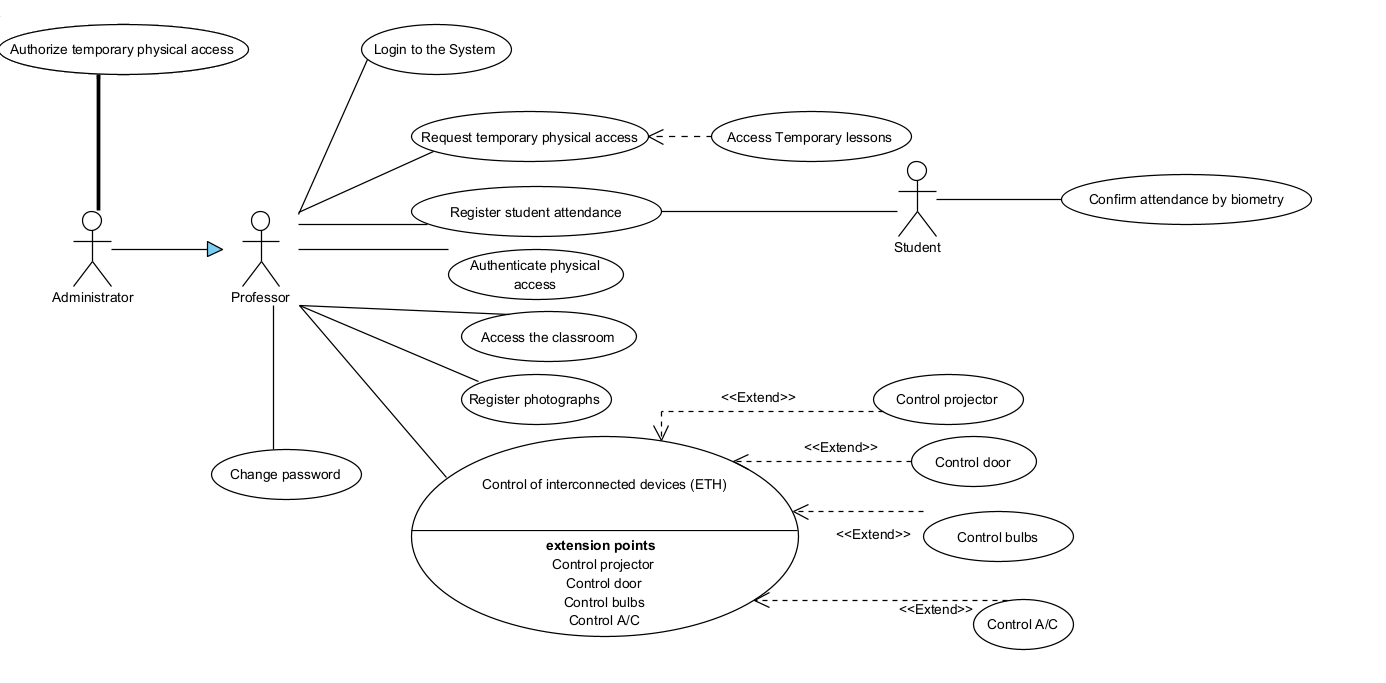
\includegraphics[scale=0.95]{useCasesDiagram.png}
            \caption{Use cases diagram of SISGERA.}
            \label{fig:useCasesDiagram}
        \end{figure}
        \note{
            Preliminary Analysis
            \textbf{Functional requirements}
            Among the main requirements to be met by SISGERA are:
            \begin{itemize}
                \item Control interconnected device: Turns on and off the lights, air conditioner and video projector.
                \item Physical access control: Verifies the identity of professor through facial recognition, and Unlocks the door to allow the professor to enter.
                \item Records student attendance by means of RFID identification.
                \item Verify the identity of students by fingerprinting.
                \item Unlock the door to let in students arriving after the start time.
            \end{itemize}
            \textbf{Non-functional requirements}
            Regarding the non-functional requirements of the system, it was determined that, as it is a system to be deployed in a classroom, the power supply is guaranteed by the public utility. As for the Internet connection, a permanent Wi-Fi connection is available.
        }
    \end{frame}
        
    \begin{frame}{Preliminary Analysis - feasibility study}
    	
        \begin{block}{Technological feasibility: IoT hardware}
            \begin{itemize}
                \item Raspberry Pi;
                \item Arduino Mega;
                \item infrared sensors;
                \item an IP camera;
                \item an RFID card reader and RFID cards;
                \item a fingerprint reader;
                \item a motion sensor; and
                \item relay modules.
            \end{itemize}
        \end{block}
    
        \note{All the IoT hardware components necessary to meet the functional requirements exist, and were within our reach.
            \begin{itemize}
                \item Raspberry Pi: for local processing and sending data via Internet.
                \item Arduino Mega: to treat the signals captured by the sensors and send the data to the Raspberry Pi through the Bluetooth module.
                \item infrared sensors: turn on and off air conditioner and video projector.
                \item an IP camera: to recognize people through live video.
                \item cards and RFID card reader: to identify students when accessing the classroom.
                \item a fingerprint reader: to identify students more securely when required.
                \item a motion sensor: to detect people presence inside the classroom; and
                \item relay modules: to turn on and off lights and equipment.
            \end{itemize}
        }
    \end{frame}
    
    \begin{frame}{Preliminary Analysis - feasibility study}
         
         \begin{block}{Technological feasibility: Software tools and technologies}
         	\begin{itemize}
         		\item Python language
         		\item Java language
         		\item Glassfish
         		\item PostgreSQL
         	\end{itemize}
         \end{block}
         
        \begin{block}{Economic feasibility}
            SISGERA is an inexpensive IoTS, it was fully funded by the project team, and its cost was within the expected budget.
        \end{block}
        \begin{block}{Operational feasibility}
            SISGERA is intended to be easy to operate.
            \begin{itemize}
            	\item RESTful web services will be created to store and retrieve the data in the database.
            	\item All universities have Academic Management Systems, which can provide the data to SISGERA.
            \end{itemize} 
        \end{block}
        \note{
            \textbf{In addition, in Technological feasibility have the Software tools and technologies}
            	\begin{itemize}
            		\item Python Language: facial recognition. Runs on Rapsberry PI
            		\item Java langauge: Mobile app, Web Services RESTfull
            		\item Glassfish applications server, and PostgreSQL: Persistence layer
            		\item PostgreSQL: Persistence layer
            	\end{itemize}
            
            \textbf{Economic feasibility}\\
            SISGERA is an inexpensive IoTS, it was fully funded by the project team, and its cost was within the expected budget.\\
        
            \textbf{Operational feasibility}\\
            SISGERA is intended to be easy to operate. RESTful web services will be created to store and retrieve the data in the database. The administrator will be able to take photographs of professors for facial recognition, and also feed the system with student and academic planning data.
    }
    \end{frame}

    \begin{frame}{Stage 2: Technology Layer Design}
        \begin{figure}
            \centering
            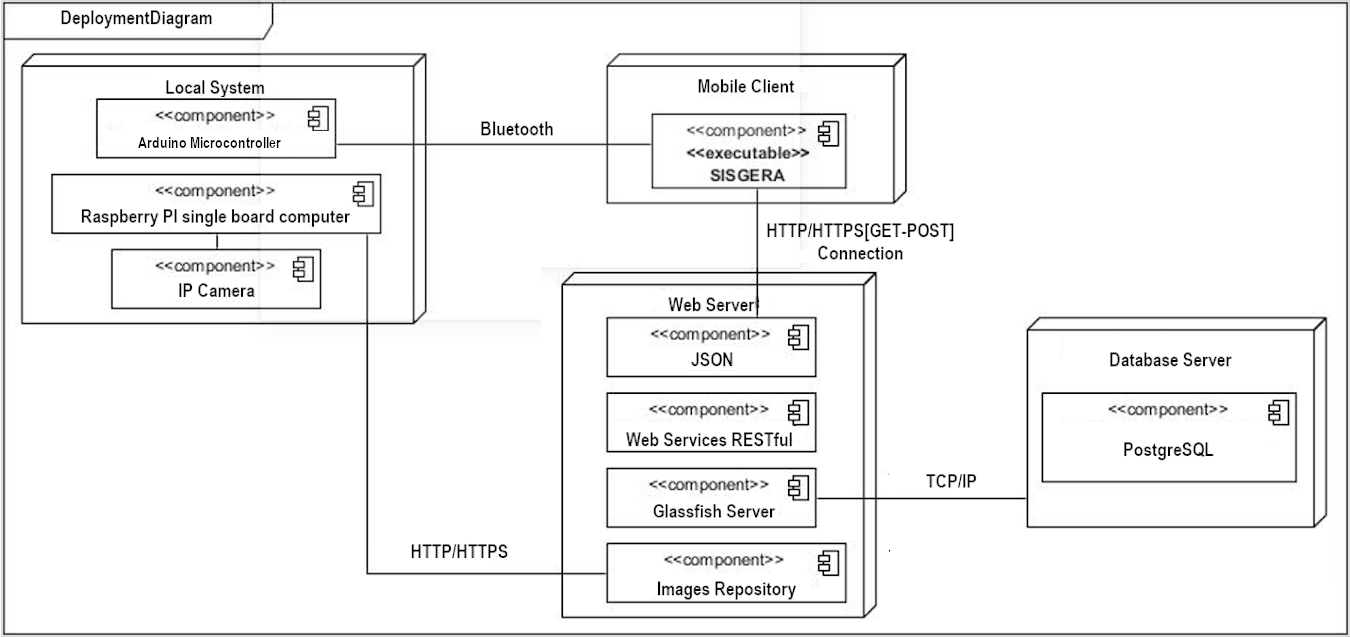
\includegraphics[scale=1.1]{architecture.png}
            \caption{SISGERA Architecture.}
            \label{fig:architecture}
        \end{figure}
        \note{
        The SISGERA architecture is designed in 4 layers:
        \begin{itemize}
            \item First layer: local processing or set of components that could be called the device,
            \item Second Layer: the mobile application with which the professor can interact with the environment,
            \item Third layer: the web server where the application server is installed, which provides the web services, and the storage of the images for facial recognition, and of course
            \item Fourth layer: the data persistence layer that basically consists of a PostgreSQL database server.
        \end{itemize}  
        }
    \end{frame}
    
    \begin{frame}{Stage 2: Technology Layer Design...}
        \begin{figure}
            \centering
            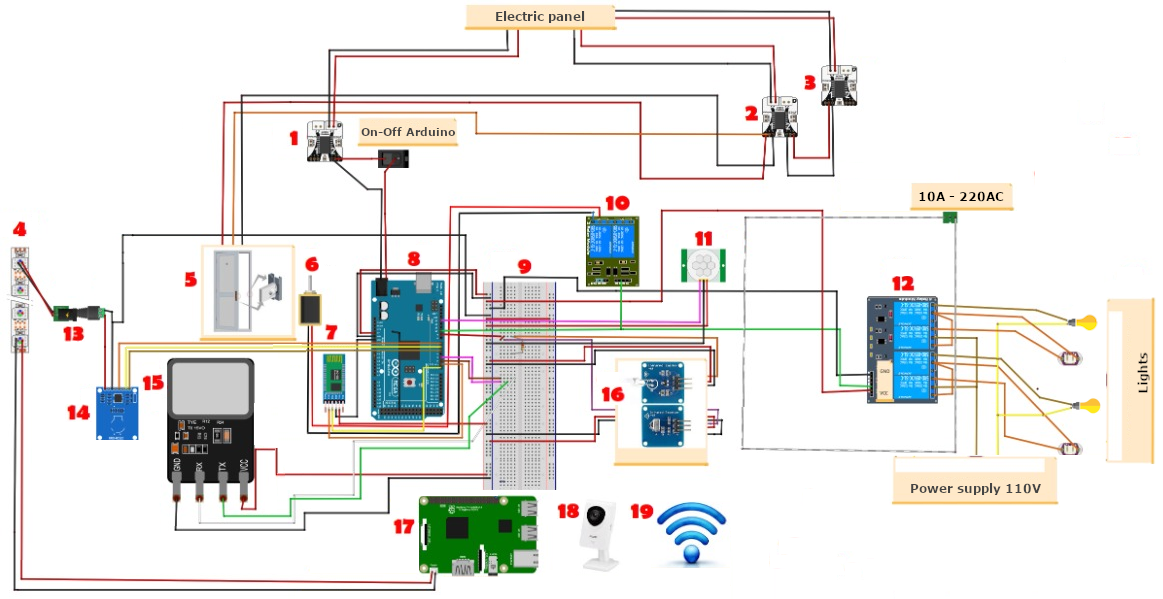
\includegraphics[scale=1.2]{deviceDiagram.png}
            \caption{IoT device design of SISGERA.}
            \label{fig:deviceDiagram}
        \end{figure}
    
    \note{
        \textbf{Components of SISGERA Device}
        \begin{multicols}{2}
                \begin{itemize}
                    \item (1) DC Breaker 220/380V,
                    \item (2) Merlin Gerin C60hb Multi9 B25 Circuit Breaker,
                    \item (3) Electric lock transformer 110V-12V,
                    \item (4) Power strip,
                    \item (5) Door control,
                    \item (6) Electric sheet DC motor,
                    \item (7) Bluetooth HC-5 module,
                    \item (8) Arduino mega 2560,
                    \item (9) Protoboard,
                    \item (10) Relay module 2 channels,
                    \item (11) HC-SR04 PIR module,
                    \item (12) 4-channel relay module,
                    \item (13) Male and female DC Power Jack Socket adapter cable,
                    \item (14) Wiegand W26 RFID reader,
                    \item (15) DFRobot fingerprint reader sensor,
                    \item (16) NE555 IR transceiver module,
                    \item (17) Raspberry Pi 4,
                    \item (18) IP camera, and
                    \item (19) Router to Wi-Fi Service.
                \end{itemize}
            \end{multicols}
            }
    \end{frame}
    
    \begin{frame}{Stage 3: Detailed requirement analysis }
        \begin{block}{Elicitation of system requirements}
            \begin{itemize}
            	\item The development of the system was divided into different deliverables and each of them was analysed.
            	\item Semi-structured use cases were used to collect those requirements.
            	\item To obtain the tests that the software must pass.
            	\item The system meets the requirements demanded by the end users.
           \end{itemize}	
    \end{block}
	\begin{block}{Semi-structured use cases}
    	Semi-structured use cases are used to describe the flow of actions that are carried out to obtain an outcome of observable value by a particular actor.
    \end{block}
    \note{
    	\textbf{Elicitation of system requirements}\\
        The development of system was divided into different deliverables. For each one, the requirements were analysed in detail to obtain the tests that the software must pass, thus ensuring that the system meets the requirements demanded by the end users. Semi-structured use cases were used to collect those requirements.
        
        \textbf{Elicitation of system requirements and Use cases}\\
        Semi-structured use cases are used to describe the flow of actions that are carried out to obtain an outcome of observable value by a particular actor.
            
        }
    \end{frame}
    
    %%\begin{frame}{Stage 3: Example of Semi-structured use case}
    %%    \begin{figure}
    %%        \centering
    %%        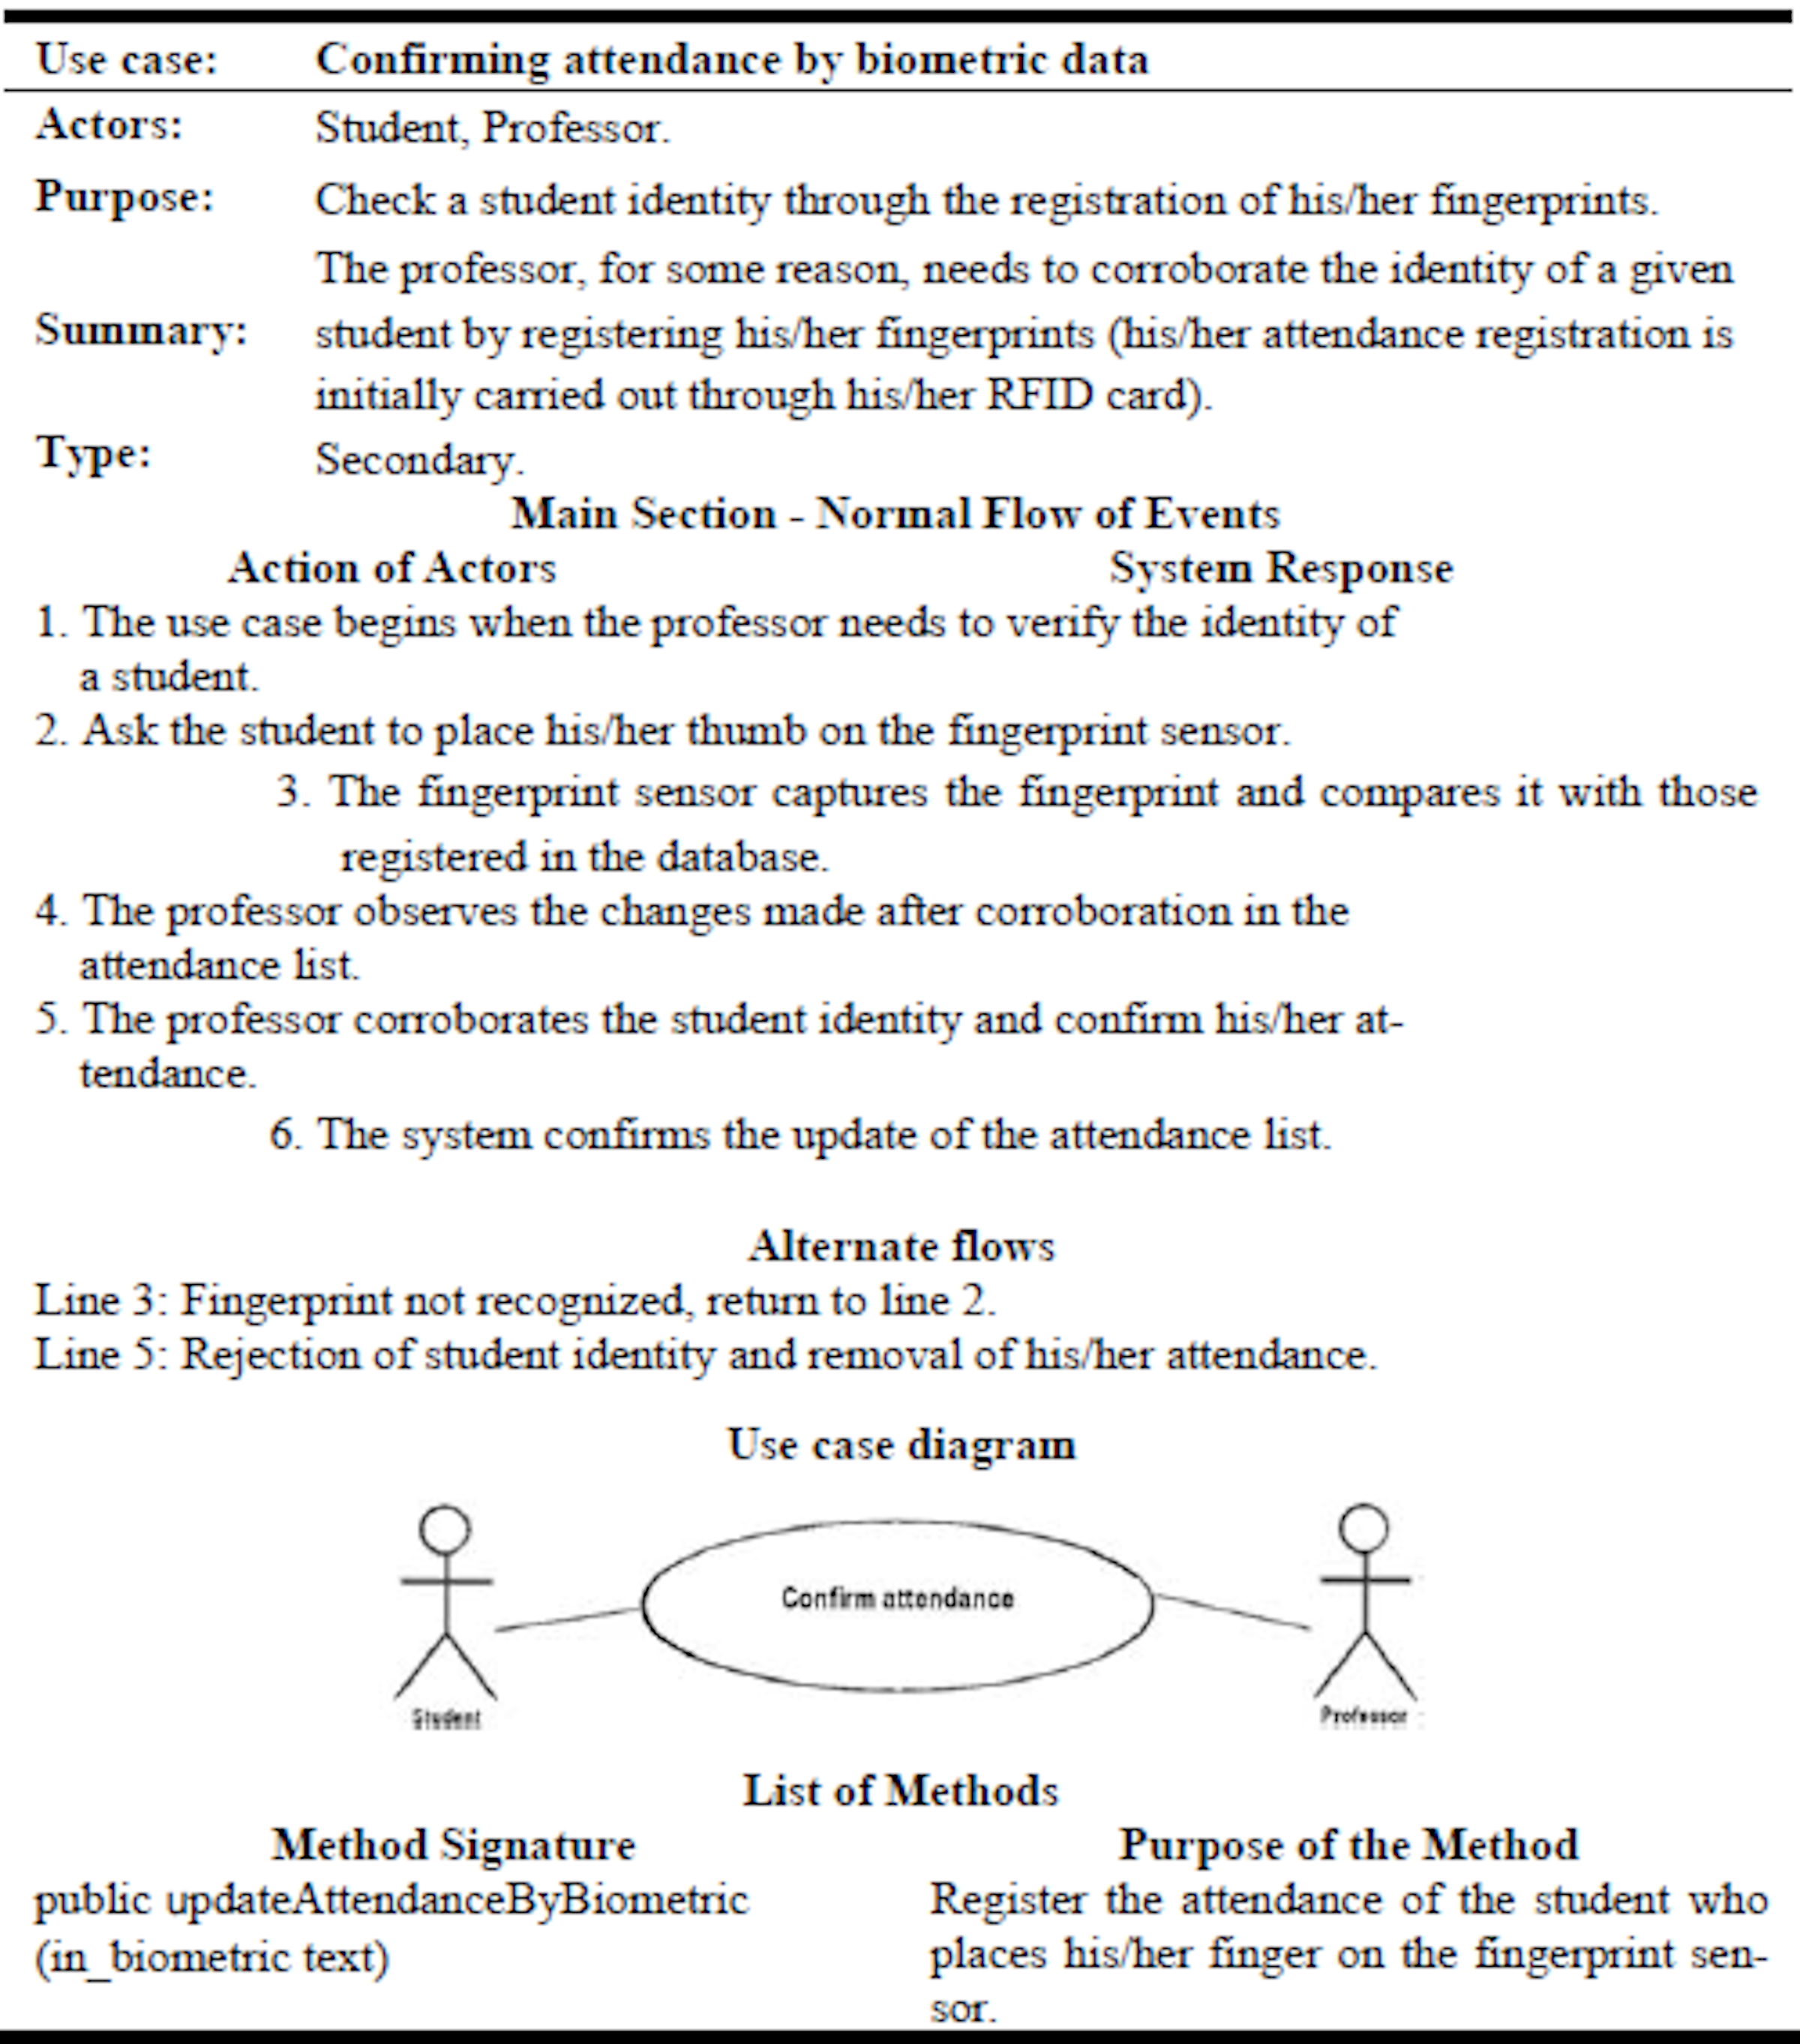
\includegraphics[scale=0.65]{useCase.png}
    %%        \caption{Confirming attendance use case.}
    %%        \label{fig:useCase}
    %%    \end{figure}
    %%\end{frame}
    
     \begin{frame}{Stage 4: Model Generation and Adaptation}
        \begin{block}{Platform-independent model}
            IoTS are heterogeneous in nature, so a platform-independent model was obtained before generating a platform-specific model.
        \end{block}
        \begin{figure}
            \centering
            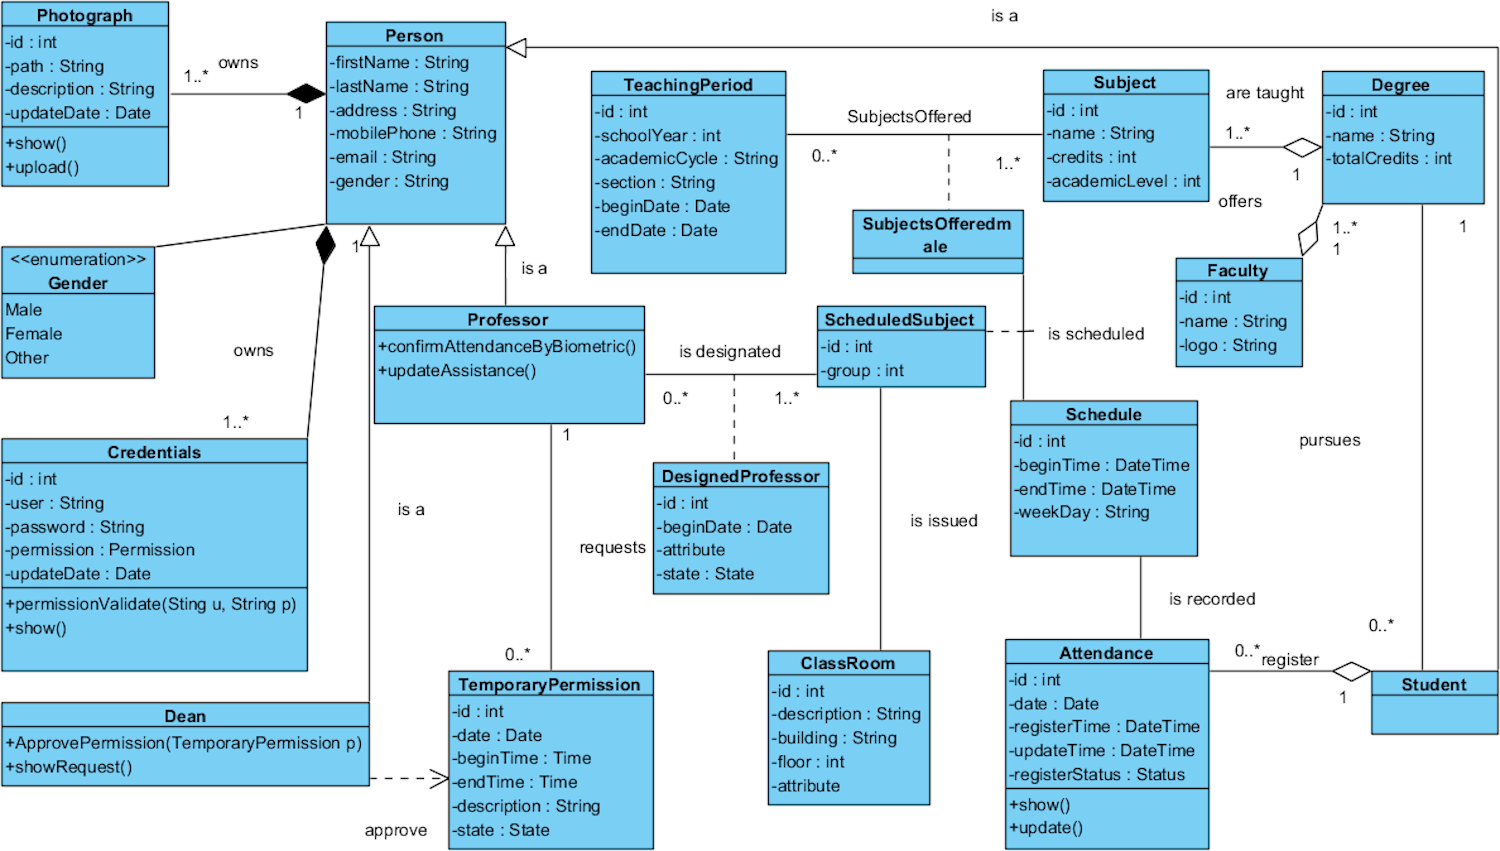
\includegraphics[scale=0.65]{classesDiagram.png}
            \caption{Class diagram of SISGERA}
            \label{fig:classesDiagram}
        \end{figure}
        \note{
            In this phase, the class diagram was created, considered one of the most important in the construction of systems, as it serves to represent the architecture of a system, and with the appropriate tools, it was used to generate the database and part of the necessary code.
        }
    \end{frame}
    
    \begin{frame}{Stage 5, 6, 7 and 8}
        \begin{itemize}
        	\item \textbf{Stage 5: Test generation:} The tests were written considering the different cases that may occur when trying to enter or leave the classroom.
        	\begin{itemize}
        		\item The professor is out of time,
        		\item he/she takes care to turn off the equipment,
        		\item etc.
            \end{itemize}
        	\item \textbf{Stage 6: Software generation}
    		\begin{itemize}
    			\item Automatic generation of the software, Visual Paradigm was used
    			\item Visual Paradigm each class with its attributes and methods
    			\item The code was used in the mobile application
    		\end{itemize}
    		\item \textbf{Stage 7: Model refinement:} This stage was not necessary
    		\item \textbf{Stage 8: Software refinement:} The guidelines for writing clean code were considered for writing the software code.
    		\begin{itemize}
    			\item It was carried out after obtaining the mobile application software for SISGERA.
    			\item The IoT hardware configuration software was not refined.
    		\end{itemize}
    	\end{itemize}
        
        \note{ 
        	\textbf{Stage 5: Test generation:}
        	The system must respond appropriately to each of the possible cases that may occur. For example: it must not allow a professor to enter if it is not his or her approved schedule. Turn on the lights and equipment when a person enters. Lights and equipment must be turned off when there are no people in the classroom.\\
           \textbf{Stage 6: Software generation:}
            This process can be manual or automatic. For the automatic generation of the software, Visual Paradigm was used. Visual Paradigm generate each class with its attributes and methods, to be used in the mobile application. 100\% of the Arduino code and the rest of the business logic code was written by the development team.\\
            \textbf{Stage 7: Model refinement:}
            This stage was not necessary because of the size of the project and the developers' mastery of the domain. This is foreseen by the authors of TDDM4IoTS.\\
        \textbf{Stage 8: Software refinement:}
            This stage was executed only once, after obtaining the mobile application software for SISGERA. It was not necessary to refine the device configuration software, as it was written considering from the beginning the guidelines to obtain a clean code.\\
        }
    \end{frame}
    
    \begin{frame}{Stage 9: Hardware and software deployment}
        \begin{figure}
            \centering
            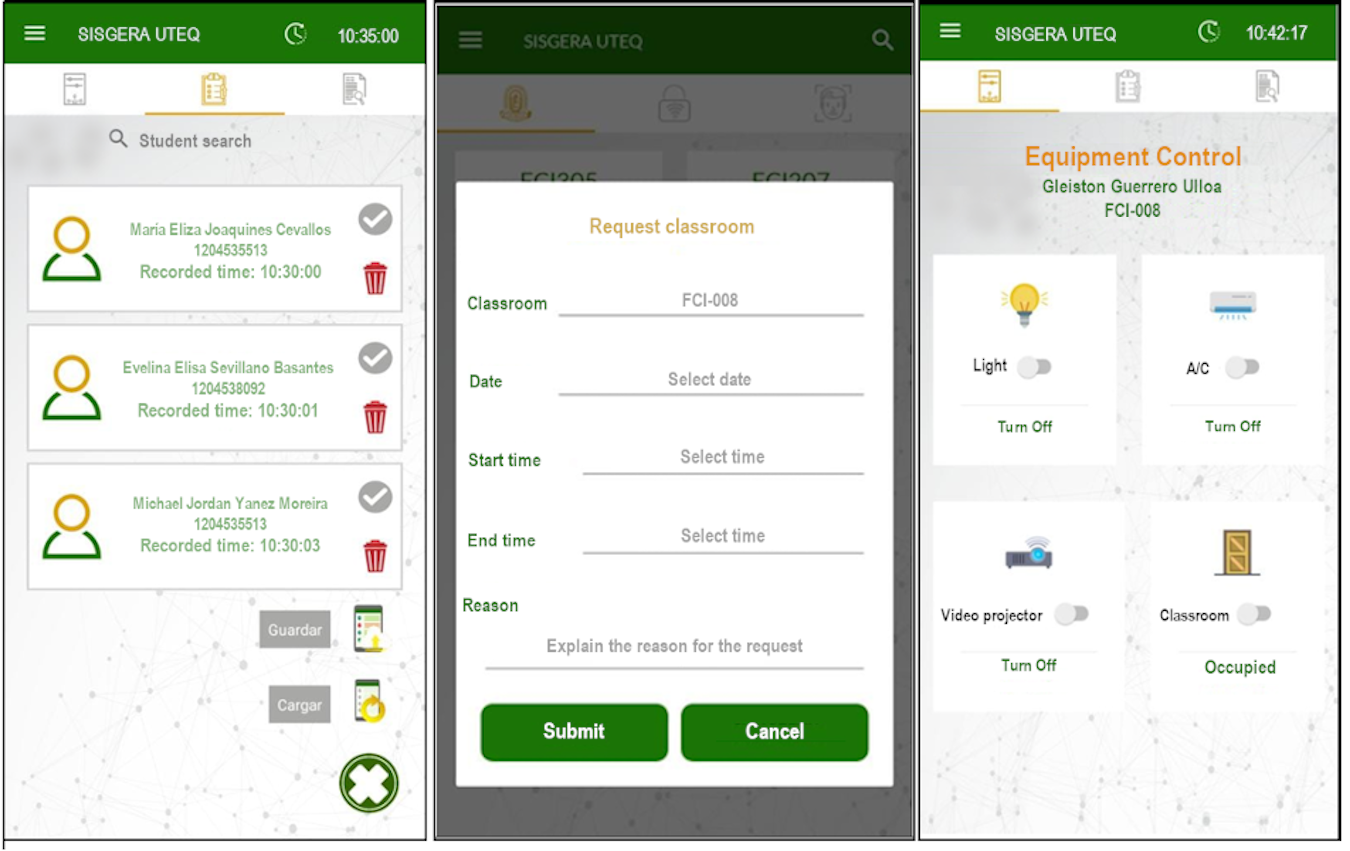
\includegraphics[scale=0.9]{mobileApp.png}
            \caption{Screenshots of the SISGERA mobile application.}
            \label{fig:mobileApp}
        \end{figure}
        \note{
            \textbf{The device} was deployed as determined in the environment analysis. It was deployed in the classroom, connecting directly to the public power supply without the need for a battery, a router was installed to fix the Wi-Fi signal with good quality.
            
            \textbf{The mobile application} was installed on the smartphones of the professors who tested the application. This application has professor and Dean roles. The latter role is the one that authorises the professor to use the requested classroom.
            
            In addition, the mobile application can be used to control all environmental devices such as lights, air conditioner, video projector, and of course the door unlocking.
        }
    \end{frame}
    
    \begin{frame}{Stage 10: Deliverable assessment}
        \begin{block}{SISGERA assessment}
            The device and the mobile application
            \begin{itemize}
            	\item Passed all tests de system acceptation.
            	\item The usability evaluation of SISGERA mobile application.
            	\item After this results, improvements were implemented. 
            	\item Those improvements resulted in 100\% acceptance by professors.
            \end{itemize} 
        \end{block}
        \begin{block}{Stage 11: Maintenance}
            The Maintenance was not carried out, due to the low complexity of the project. Moreover, it is a prototype that is to be evaluated.
        \end{block}
        
        \note{
            \textbf{Stage 10: SISGERA assessment}\\
            The device and the mobile application passed all tests specified in the test generation stage. In addition, the usability evaluation of SISGERA was done along 5 weeks only by professors. Following these results, more professors were involved in the design of the mobile application interfaces, to implement improvements. Those improvements resulted in 100\% acceptance by professors.

        \textbf{Stage 11: Maintenance}\\
            SISGERA is a prototype, but considering the improvements made by the professors' comments, maintenance was not carried out as it is not a production system. However, it is planned to put it into production for a more exhaustive evaluation and to consider the maintenance stage.
        }
    \end{frame}
    
\section{Conclusion}
    \begin{frame}{Conclusion}
        \begin{itemize}
            \item We have presented SISGERA, an IoTS for classroom access control and resource management. It uses facial recognition for professors, and fingerprint recognition and RFID for students as user authentication methods.
            \item SISGERA is designed to be replicated in different classrooms.
            \item TDDM4IoTS is an effective guide for IoTS developers.
            \item End-users should maintain a dedicated involvement in the development of the IoTS.
            \item As future work, the usability of the application by students and the energy consumption of two different classrooms.
        \end{itemize}
        \note{
            \textbf{Conclusion}
            \begin{itemize}
                \item We have presented SISGERA, an IoTS for classroom access control and resource management. It uses facial recognition for professors, and fingerprint recognition and RFID for students as user authentication methods.
               
                \item The combination of RFID authentication and fingerprint recognition as identification methods can be used to deter students from identity theft.
                \item SISGERA is designed to be replicated in different classrooms as a distributed system.
                \item La reduction in energy consumption can be calculated according to the time that the equipment are kept off.
                \item TDDM4IoTS is an effective guide for IoTS developers, especially for those who do not have sufficient experience in IoTS development.
                \item End-users should maintain a dedicated involvement in the development of the IoTS, especially in the design of its user interfaces.
                TDDM4IoTS encourages user participation from the earliest stages of IoTS development.
                \item As future work, the usability of the application by students and the energy consumption of two different classrooms, with and without the SISGERA system, respectively, will be evaluated.
            \end{itemize}
        }
    \end{frame}
\section*{Acknowledgement}  
\begin{frame}
\textcolor{myNewColorA}{\Huge{\centerline{Thank you!}}}
\end{frame}

\end{document}



